\section{Algorithms Implemented in \EASAL}
\label{sec:algorithms}

\begin{figure}
\centering
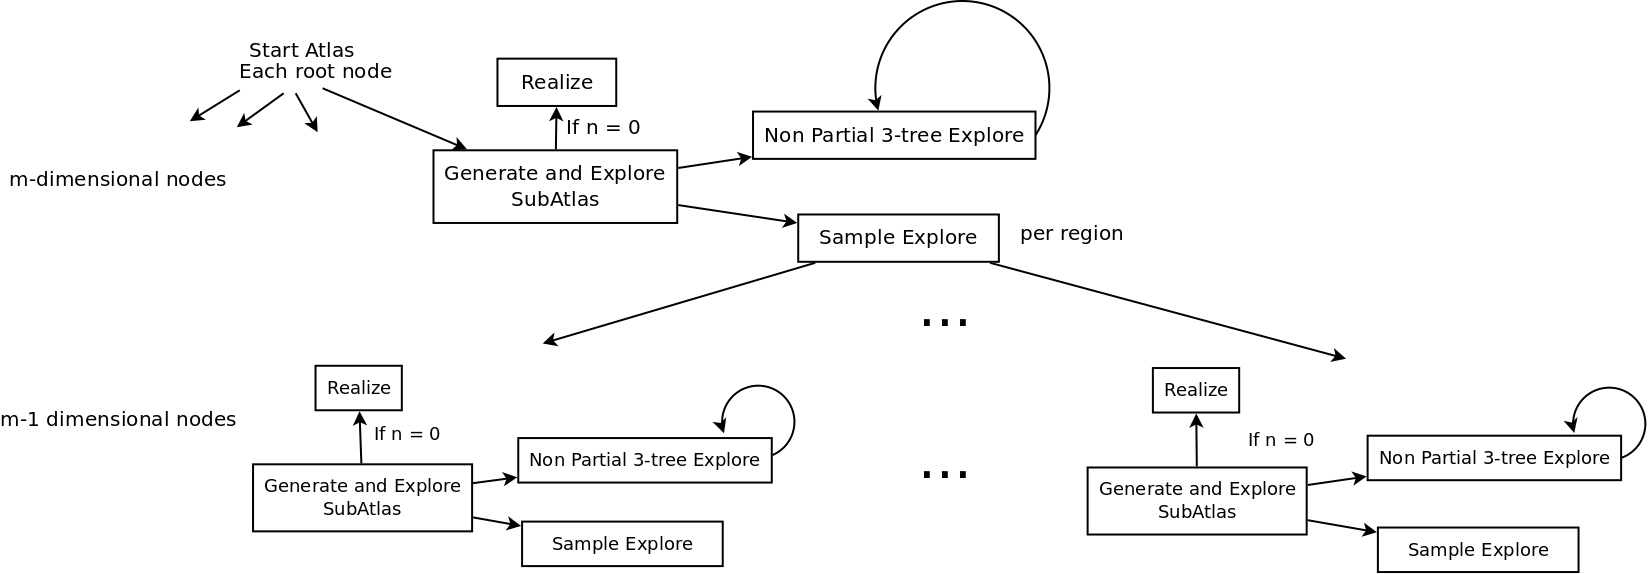
\includegraphics[width=\textwidth] {\fig/Algorithm.png}
\caption{Algorithm for generating and exploring the atlas}
\label{fig:algorithm}
\end{figure}


\textbf{Stratification}:
This algorithm captures, stores, and labels the stratification regions of the
configuration space. The regions of the atlas are stored as nodes of a
directed acyclic graph (\figref{fig:natlas} and \figref{fig:flips}), whose
edges represent immediate containment or reachability. Each region of the
atlas is identified by a (small) \textit{activeConstraintGraph} $G_H$ where $H$
is the set of active constraints. A newly discovered $G_H$ is tested to ensure
that it is not already present in the current \emph{atlas}. Only if $G_H$ is
new the region is further explored; by default, this is done depth first. New
active constraints and regions are added individually by sampling the space at
a user specified level of refinement.


\textbf{Cayley Sampling}:
\figref{fig:algorithm} gives an overview of how sampling and exploration is
done in \EASAL.  We sample the active constraint regions via grid sampling in the
Cayley parameter grid to define the grid. In addition we use binary search near
the boundary to discover lower dimensional boundary regions where new
constraints become active as described under `Detect Active Constraint'. We
determine the parameter set $F$ of the active constraint graph that yields a
partial 3-tree. We then compute the range of $F$ for the active constraint
region.



\textbf{Convex Parametrization}:
The parameters $F$ of an active constraint graph are selected so as to form a maximal
3-tree to leverage the convex parametrization
theory~\cite{Gao}. The algorithm works by searching a superset of the active
constraints of the graph from the list of complete 3-trees in
\figref{fig:3-trees}. For this purpose a look-up table is created, that holds
all complete 3-trees. Searching is done among all isomorphisms of the graphs of
complete 3 trees. If a superset is found then the edges in that graph (except
the active constraints) will be used as the parameter set.

\textbf{Chart Range Computation}: If Convex Cayley parametrization theory is
applicable to the active constraint graph, then the chart that is defined by
the set of Cayley points traced out by the Cayley parameters happens to be
convex. In other words, the active constraint graph has a convex Cayley
configuration space if it is a partial 3-tree. Then we need to compute the
bounds of the convex region where the sampling occurs and prevent the sampling
from going beyond the feasible region. Finding bounds for each non-edge has two cases
and the range computation for each of these cases is handled as follows:
\begin{itemize}
		\item When there is only one parameter in a tetrahedron and all the
				other edges are fixed, the range of that parameter can be
				computed by the intersection of the triangular and tetrahedral
				inequalities.
		\item If there is more than one unfixed parameter in the tetrahedron,
				then the range of all parameters except one will be computed
				through triangular inequalities and fixed by assigning a value
				within their range. Then the range of the one remaining
				parameter will be computed as in the first case through both
				triangular and tetrahedral inequalities. Since the range of
				the parameter is affected by the previously fixed parameters,
				range computation of the unfixed parameter is required
				for every iteration/assignment of fixed parameters.
\end{itemize}

\textbf{Ordering of Parameters}: Fixing a non-edge requires the range
computation for the non-fixed parameter that takes place in the same
tetrahedron. The order in which this is done has an effect on the efficiency
of sampling~\cite{ugandhar}. This algorithm picks the parameters in the order
that gives the best efficiency.

%--------------------
\textbf{Detect Active Constraint}: Detects a newly active constraint and a new
region of the stratification in a smaller dimensional stratum. \EASAL~relies on
grid sampling on the Cayley grid to find the children of each active constraint
region and uncover the topology of the atlas by exhaustively exploring
boundaries with a certain step size. When a new active constraint is detected
via binary search described under `Cayley Sampling', the regions of its children
are recursively sampled and explored.



However, boundary detection is not guaranteed by grid sampling alone. The
threshold may not be large enough to allow the Constraint Check algorithm to
define a close by atom pair to be a distance constraint, i.e., edge of the
active constraint graph. Furthermore, neighboring Cayley points may be in
violation of steric or hard sphere constraints. As a result, the boundary
region would be missed since it is located in between a feasible point and a
point violated by sterics. Exploration (by the way of binary search) is
required to find any additional constraints that restrict the region, e.g.\
steric constraints that render a configuration infeasible.

\begin{figure}
\centering
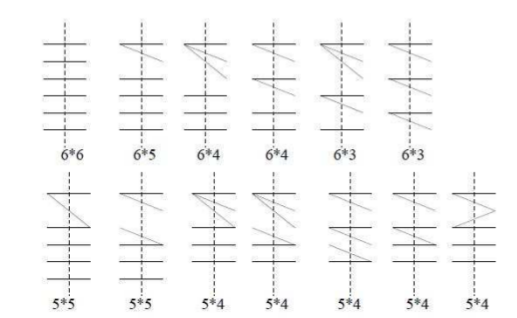
\includegraphics[scale=0.25] {\fig/partial3tree_new.png}
\caption{All 3-tree active constraint graphs for $k = 2$ rigid bodies in $R^3$.
It should be noted that the vertices on the left and the right of this graph
form a complete graph(edges not shown) since the atoms on each node belong to a
rigid unit.  The label $m_1$ $m_2$ below each active constraint graph indicates
that $m_1$ atoms in $M_1$ are connected to $m_2$ atoms in $M_2$ . Solid edges
indicate pairs whose distance is fixed matching their Lennard-Jones potential.}
\label{fig:3-trees}
\end{figure}

\textbf{Cartesian Realization}: To find the Cartesian realization we add one
atom at a time using distances from already realized atoms to get a partial
3-tree. This gives us a convex space TODO:and in addition finding a realization is
easier than the general Cartesian realization problem. For nodes of
dimensions 3 and higher, it is always guaranteed that we will get a convex
region.
TODO: Reorg it better
For 1D and 2D regions, i.e., 4 or 5 constraints are active, where it is
sometimes not a partial 3-tree and hence a convex region,
we drop a constraint and explore a higher dimensional region using ray
tracing to compute the Cartesian realization.


